\section{Data}
\label{sec:data}
The dataset used was a mix of the CrowdFlower 
dataset\cite{crowdflower_dataset} and the
Emotions dataset\cite{emotions_dataset}.
The CrowdFlower dataset contains 40,000 tweets
labeled with 13 different emotions. The Emotions 
dataset contains 400,000 tweets labeled with 6 
different emotions.

\subsection{Exploratory data analysis and preparation}
Some emotions that are present in the
CrowdFlower dataset were remapped because they
were too similar to other emotions and 
would make the classification task harder.
The emotions and relative mappings are:
\begin{itemize}
    \item Happiness
    \item Sadness
    \item Anger
    \item Worry
    \item Love
    \item Surprise
    \item Neutral
    \item Fun $\rightarrow$ Happiness
    \item Relief $\rightarrow$ Happiness
    \item Hate $\rightarrow$ Anger
    \item Empty $\rightarrow$ Neutral
    \item Enthusiasm $\rightarrow$ Happiness
    \item Boredom $\rightarrow$ Neutral
\end{itemize}

\begin{figure}[H]
    \centering
    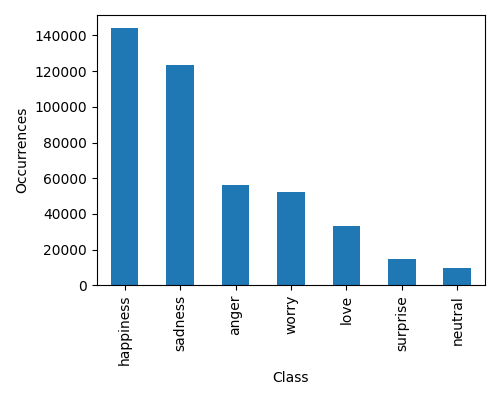
\includegraphics[width=0.48\textwidth]{images/class_distribution.png}
    \caption{Class distribution of the full dataset}
    \label{fig:class_distribution}
\end{figure}

As shown in \autoref{fig:class_distribution},
the dataset is imbalanced. The most common
emotion is Happiness, and the least common
is Neutral. This is because the larger dataset
(Emotions) does not contain the Neutral class.

\begin{figure}[H]
    \centering
    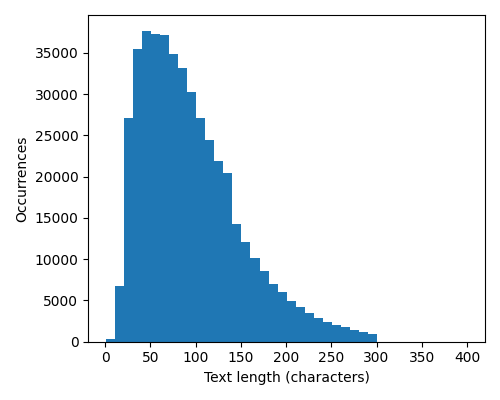
\includegraphics[width=0.48\textwidth]{images/length_distribution.png}
    \caption{Text length distribution of the full dataset}
    \label{fig:length_distribution}
\end{figure}

The dataset was split into a training set
and a test set with a 80\% - 20\% ratio.

\subsection{Preprocessing}
Multiple kinds of preprocessing were tested:
\begin{itemize}
    \item \textit{Bag of words (BoW)}
    \item \textit{Word embeddings (WE)}
    \item \textit{GloVe embeddings (GE)}
\end{itemize}
For the BoW and WE preprocessing, the text was
first cleaned with a regular expression that
removes urls, mentions and symbols. Then the
text was tokenized and stemmed with the 
Snowball stemmer. Both \textbf{TFIDF} and 
\textbf{binary} encodings were tested for
the BoW preprocessing.
The GE preprocessing was done by applying 
the same cleaning regular
expression but without stemming. The vectors
used were the 6B 50d vectors from
GloVe\cite{glove}.
The main difference between the WE and GE
preprocessing is that the WE vectors were
trained on the dataset, while the GE vectors
were pre-trained on a large corpus of text.
